\title{EE660 Project Report}
\author{
        Vinaykumar Hegde \\
        USC ID: 4809250026 \\
%                Department of Electrical Engineering\\
%              University of Southern California\\
%        Los Angeles, CA - 90007, \underline{USA}
}
\date{\today}


\documentclass[12pt]{article}

\usepackage[square,sort,comma,numbers]{natbib}
\bibliographystyle{plainnat}
\usepackage{float}
\usepackage{amssymb}
\usepackage{amsmath}
\usepackage{hyperref}
\usepackage{graphicx} 
 
\usepackage{geometry}
\geometry{
 letterpaper,
 left=30mm,
 top=30mm,
}
\usepackage{fancyhdr}
\pagestyle{fancy}
\lhead{EE660: Project Report}
\rhead{Vinaykumar Hegde}

\renewcommand*\contentsname{Table of Contents}

\begin{document}
%%%%%%%%%%%%%%%%%%%%%%%%%%%%%%%%%%%%%%%%%%%%%%%%%%%%%%%%%%%%%%%%
\begin{titlepage}
\begin{center}

% Upper part of the page. The '~' is needed because \\
% only works if a paragraph has started.
%\includegraphics[width=0.15\textwidth]{./logo}~\\[1cm]

\textsc{\LARGE University of Southern California}\\[1.5cm]

\textsc{ EE660: Machine Learning from Signals: Foundations and Methods}\\[0.5cm]

% Title
%\hrule \\[0.4cm]
~\\[2cm]
\hrule
~\\[0.2cm]
{ \LARGE \bfseries CIFAR-10: Object Detection in Images\\[0.4cm] }
\hrule
%\hrule \\[1.5cm]
~\\[3.5cm]

% Author and supervisor
\noindent
\begin{minipage}{0.9\textwidth}
\begin{flushleft} \large
\emph{\underline{Submitted By:}}\\
Vinaykumar S. Hegde\\
Graduate Student\\
Department of Electrical Engineering.\\
University of Southern California, CA\\
USC ID: 4809250026\\
USC email: vinaykuh@usc.edu\\
Submission Date: Dec 8, 2015 \\
\end{flushleft}
\end{minipage}%
\begin{minipage}{0.55\textwidth}
%\begin{flushright} \large
%\emph{\underline{Advisor:}} \\
% Prof, details.
%\end{flushright}
\end{minipage}

\vfill

% Bottom of the page
%{\large \today}

\end{center}
\end{titlepage}


%%%%%%%%%%%%%%%%%%%%%%%%%%%%%%%%%%%%%%%%%%%%%%%%%%%%%%%%%%%%%%%%
\tableofcontents

%%%%%%%%%%%%%%%%%%%%%%%%%%%%%%%%%%%%%%%%%%%%%%%%%%%%%%%%%%%%%%%%
\section{Project Homepage}
CIFAR-10: Object Recognition in Images\\
Bigbucket Page: 

\url{https://bitbucket.org/vinaykumarhs2020/ee660\_project}



%%%%%%%%%%%%%%%%%%%%%%%%%%%%%%%%%%%%%%%%%%%%%%%%%%%%%%%%%%%%%%%%
\section{Abstract}
CIFAR-10 is a tiny image dataset is provided by \citet{ref:dataset} of University of Toronto. This has 60,000 32x32 RBG images are divided into 50,000 train and 10,000 test images. This dataset is smaller compared to other object detection datasets, but equally challenging because of very small size of the images.

This project aims at applying machine learning techniques to classify images into 10 different categories: airplane, automobile, bird, cat, deer, dog, frog, horse, ship, truck. First major part of the project is feature extraction and next part is the model selection for machine learning algorithms. Features extractions like \textbf{H}istogram \textbf{o}f \textbf{G}radients (HOG),\textbf{B}ag \textbf{o}f \textbf{W}ords/\textbf{F}eatures  (BOW/BOF) of \textbf{S}cale \textbf{I}nvariant \textbf{F}eature \textbf{T}ransform(SIFT) are tried with \textbf{S}upport \textbf{V}ector \textbf{M}achines (SVM) and \textbf{R}andom \textbf{F}orest techniques. In the last part of the project, \textbf{C}onvolutional \textbf{N}eural \textbf{N}etwork (CNN) is explored and seems to give very good result with this dataset.

Out of all the classifiers, CNN performs the best with 78\% accuracy on testing data (and 82\% accuracy on training data). Next best result is SVM classifier with HOG features. This accuracy is almost half of CNN accuracy. 42\% on training set. SVM results are from obtained from cross validation and grid search over wide range of parameters. 

\begin{figure}[H]
\centering
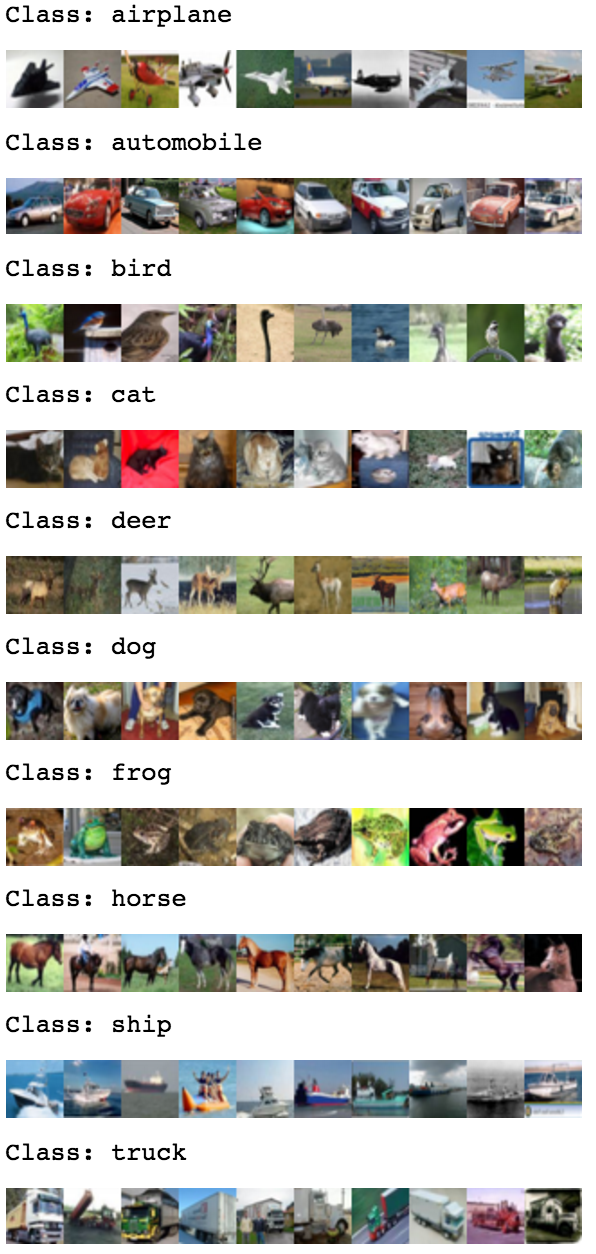
\includegraphics[width=0.5\textwidth]{images/dataset.png} 
\caption{Example images in CIFAR-10 Dataset}
\label{img:dataset}
\end{figure}

%%%%%%%%%%%%%%%%%%%%%%%%%%%%%%%%%%%%%%%%%%%%%%%%%%%%%%%%%%%%%%%%
\section{Problem Statement and Goals}
This project aims at evaluating various machine learning techniques for object detection in images, specifically in tiny images. Inherently image classification is non trivial because of various reasons. Pixel values themselves are not good set of features. Alex \cite{ref:dataset} shows that pixel values are higly correlated and need transformations or whitening operations to remove the correlation. Even then, number of pixels in image might exceed several thousands and burst the number of features in training.

These is an engineering problem and can be solved by better feature extraction techniques. Some of the common image features extractions depend on corner values, gradients and other variations in the image. Extracted features can be provided to classifiers, like SVM or Random Forest to classify the images. 

Aim of this project is to compare the performance of these algorithms on features extracted from images and try to explore other methods to improve the performance.





%%%%%%%%%%%%%%%%%%%%%%%%%%%%%%%%%%%%%%%%%%%%%%%%%%%%%%%%%%%%%%%%
\section{Literature Review}
Feature extraction form image is the crucial step of this project. Several image feature extraction techniques are explored and tested on SVM and Random Forest Classifiers.
\subsection{Bag of Features (BOF)}
This is derived from text classification literature (Bag of Words) and based on histogram of keywords in the document. \citet{ref:bof} showed the efficient method of creating bag of image keypoints and using the generated histogram as features for visual categorization. This method can be summarized as:
\begin{enumerate}
\item Find the image keypoints (SIFT, SURF or ORB)
\item Get the image descriptors for the detected keypoints
\item Cluster the keypoints into k clusters - representing k words.
\item Create a histogram of features and normalize it.
\end{enumerate}
This histogram is used as features for image classification. 
\subsubsection*{Image Keypoints and Descriptors }\label{sec:bof_lit}
Popular keypoint descriptors are Scale Invariant Feature Descriptors (SIFT) \cite{ref:sift}, Speeded-Up Robust Features \cite{ref:surf} and, Oriented FAST and Rotated BRIEF (ORB) \cite{ref:orb}. All of these methods are explored and SIFT is the only method that is found to work faithfully. SURF and ORB need 32x32 window around the keypoints to define the descriptors. Since the CIFAR-10 dataset is tiny (32x32), extracting SURF and ORB descriptors seems to be difficult, unless we make some algorithmic changes.

Several parameters settigns in SIFT are explored and Number Octaves = 4, Contrast Threshold = 0.01,  Edge Threshold = 20, Sigma=1.2 are found to work well. Default parameters proposed by \citet{ref:sift} has Sigma = 1.6 and this configuration doesn't seem to work on our dataset. With default settings, 96 train images and 24 test images were without even single features. With my setting, only 2 train images had no features and all test images had at least one features.  

\subsection{Histogram of Gradients(HOG)}\label{sec:hog_lit}
Histogram of Gradients (HOG) was proposed by \citet{ref:hog} in \citeyear{ref:hog} as an alternative to SIFT in pedestrian detection algorithm. This features can also be used for other application because of their versatility and dense nature. Unlike SIFT, these are dense features and whole image is considered while extracting features. 

Image is divided down into several cells of fixed size and blocks are defined as some combination of these cells. Blocks stride may have overlap. Histogram of gradients are calculated for each of these blocks and quantized into 8 or 9 bin values corresponding to angle ranges. For this project, Scikit-Image \cite{ref:scikit-image} was used to extract HOG features and configurations used are:  9 orientations,  8x8 pixels per cell,  3x3 cells per block.

\subsection{Convolutional Neural Network(CNN)}\label{sec:cnn_lit}
While the image feature extractions depend on handcrafted/user defied parameters, modern object detection techniques use features learnt from dataset using several iterations and convolution with trained filters. This technique was introduced by \citet{ref:lecun} in \citeyear{ref:lecun} and gained momentum after PASCAL and Imagenet challenges. AlexNet \citep{ref:alexnet} and VGGNet \citep{ref:vggnet} are two popular architectures which have won Imagenet competitions previously and used widely in object detection applications. AlexNet is dense, shorter and uses larger convolutional filters. VGGNet, on the other hand, uses smaller convolutions and much deeper. Both are known to produce very very good results compared to any conventional machine learning algorithms. It is also common to use trained VGGNet or AlexNet as feature extractors and tap the intermediate layer outputs to get the features for images. Forward propagation is very quick and can be a very efficient feature extractor. Figure \ref{img:alexnet} shows the architecture of AlexNet.
\begin{figure}[H]
\centering
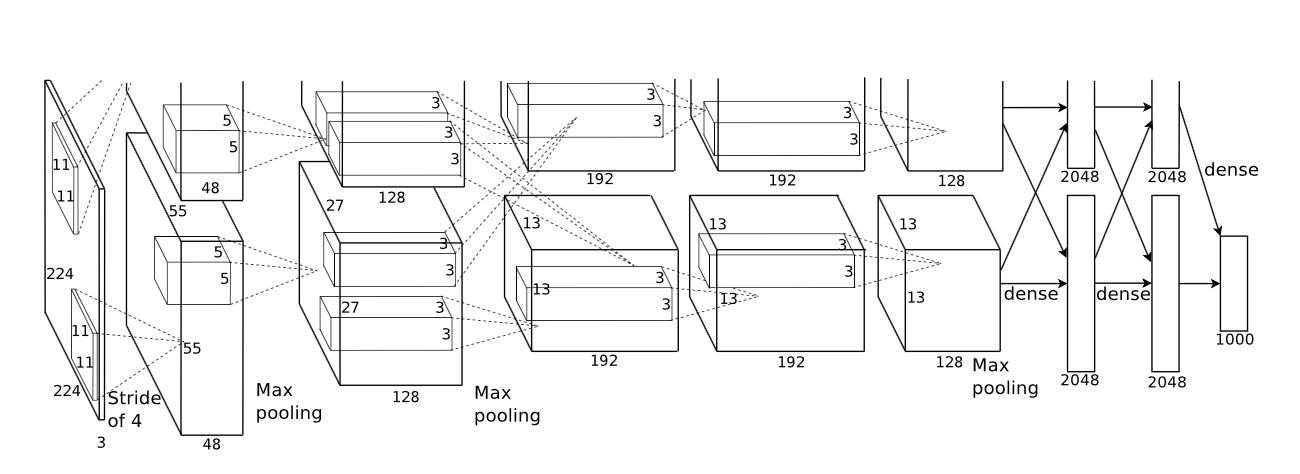
\includegraphics[width=0.9\textwidth]{images/alexnet.png} 
\caption{Architecture of AlexNet}
\label{img:alexnet}
\end{figure}

%%%%%%%%%%%%%%%%%%%%%%%%%%%%%%%%%%%%%%%%%%%%%%%%%%%%%%%%%%%%%%%%
\section{Prior and Related Work}
This project is done independently and does not coincide with any current or prior works.




%%%%%%%%%%%%%%%%%%%%%%%%%%%%%%%%%%%%%%%%%%%%%%%%%%%%%%%%%%%%%%%%
\section{Project Formulation and Setup}
Algorithm details, parameters to tune, flowchart and formulas

\subsection{Support Vector Machines (SVM)}
SVM Classifiers are very well known in machine learning and found to yield very good results. Using appropriate kernels and parameters, we can achieve very good results. Idea of using this classifier for image object detection is very old and was also published by \citet{ref:hog} in \citeyear{ref:hog}. This motivated me to try it on CIFAR-10 dataset and test the performance. Figure \ref{img:flowchart_learning} shows the flowchart for my implementation. 

\begin{figure}[H]
\centering
%%\documentclass{article}

%\usepackage[latin1]{inputenc}

%\begin{document}

\pagestyle{empty}


% Define block styles
\tikzstyle{decision} = [diamond, draw, fill=blue!20, 
    text width=4.5em, text badly centered, node distance=3cm, inner sep=0pt]
\tikzstyle{block} = [rectangle, draw, fill=blue!20, 
    text width=5em, text centered, rounded corners, minimum height=4em]
\tikzstyle{line} = [draw, -latex']
\tikzstyle{cloud} = [draw, ellipse,fill=red!20, node distance=3cm,
    minimum height=2em]
    
\begin{tikzpicture}[node distance = 2cm, auto]
    % Place nodes
    \node [block] (init) {initialize model};
    \node [cloud, left of=init] (expert) {expert};
    \node [cloud, right of=init] (system) {system};
    \node [block, below of=init] (identify) {identify candidate models};
    \node [block, below of=identify] (evaluate) {evaluate candidate models};
    \node [block, left of=evaluate, node distance=3cm] (update) {update model};
    \node [decision, below of=evaluate] (decide) {is best candidate better?};
    \node [block, below of=decide, node distance=3cm] (stop) {stop};
    % Draw edges
    \path [line] (init) -- (identify);
    \path [line] (identify) -- (evaluate);
    \path [line] (evaluate) -- (decide);
    \path [line] (decide) -| node [near start] {yes} (update);
    \path [line] (update) |- (identify);
    \path [line] (decide) -- node {no}(stop);
    \path [line,dashed] (expert) -- (init);
    \path [line,dashed] (system) -- (init);
    \path [line,dashed] (system) |- (evaluate);
\end{tikzpicture}


%\end{document}
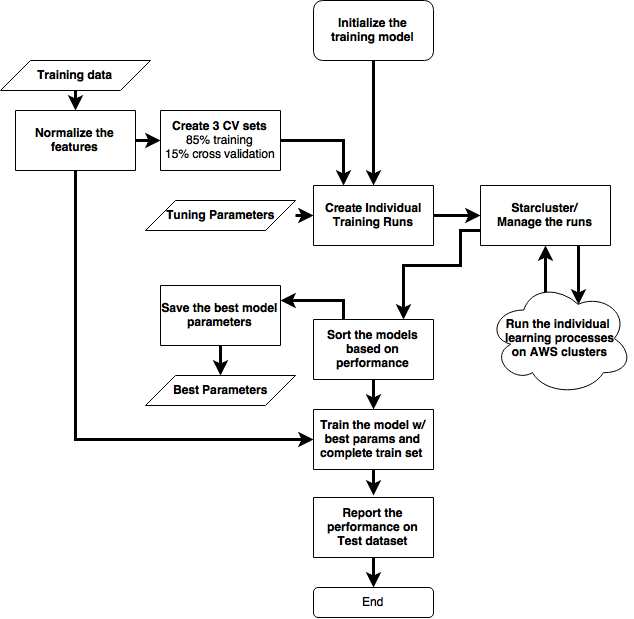
\includegraphics[width=0.8\textwidth]{images/flowchart_learning.png} 
\caption{Flowchat - Model Selection Algorithm}
\label{img:flowchart_learning}
\end{figure}

\subsubsection*{Mathematic Formulation}
Let $y_i$ represent the class of image $i$ represented by feature vector $\textbf{x}_i$. Since we have 10 classes, we can use any multi-class approaches like one-vs-all method to classify them. This breakdown the problem to binary case and now let $y_i \in \{-1,1\}$ represent if the example belongs to class $i$ ($y_i = 1$) or not ($y_i=-1$). Let $\textbf{w}$ be the weights and $b$ be the constant term. Main objective in SVM is to minimize number of classification errors by finding a decision boundary that minimizes:  $ ||\textbf{w}|| $ subject to  $y_i (\textbf{w}.\textbf{x}_i - b) \geq 1 $. If the data is not linearly separable, we can use some other kernels to classify the data.
\subsubsection*{Parameters to be tuned}
In this project, I am using Scikit-Learn's \cite{ref:scikit} SVC implementation (which is a python wrapper over libSVM), to classify the data. Following parameters can be tuned to achieve better results:
\begin{itemize}
\item \textbf{C}: Penalty parameter of error term.
\item \textbf{kernel}: Type of kernel to be used (linear, rbf)
\item \textbf{gamma}: Kernel coefficient in rbf kernel
\end{itemize}

\subsection{Random Forests and AdaBoost}
Random Forests are well know ensemble learning algorithms where multiple decision trees are constructed during training and test data is classified based on mode of decisions given by individual decision trees. This uses the concept to bagging to select random features during training. AdaBoost, on the other hand, is a meta algorithm, which can be used in conjunction with any decision trees algorithms to classify the data. AdaBoost with decision trees is know best out-of-the-box classifier with very few parameters to be tuned.

This project aims to combine AdaBoost with Random Forest for image classification. Simplicity and quick results of these classifiers motivated me to use in the project. Figure \ref{img:flowchart_learning} shows the flowchart of implementation.

\subsubsection*{Parameters to be tuned}
Scikit-Learn provides python implementations of both, Random Forests and AdaBoost. Following are the parameters to be tuned:
\begin{itemize}
\item \textbf{max depth}: depth of decision trees
\item \textbf{max features}: number of features to consider during split.
\item \textbf{n estimators}:  max number of estimators at which boosting is terminated.
\item \textbf{learning rate}: shrinkage of contribution of individual classifier.
\end{itemize}

\subsection{Convolutional Neural Networks}
Figure \ref{img:cnn_arch} represents the cnn architecture used in this project. This is a very small network compared to any other popular networks like AlexNet, VGGNet or GoogLeNet. This architecture is borrowed from Keras\citep{ref:keras}/Theano example implementation. Table \ref{tab:cnn_layers} shows the layer parameters in this project and Figure \ref{img:cnn_arch} shows the layer connections. 
\begin{figure}[H]
\centering
%%\documentclass{article}

%\usepackage[latin1]{inputenc}

%\begin{document}

\pagestyle{empty}


% Define block styles
\tikzstyle{decision} = [diamond, draw, fill=blue!20, 
    text width=4.5em, text badly centered, node distance=3cm, inner sep=0pt]
\tikzstyle{block} = [rectangle, draw, fill=blue!20, 
    text width=5em, text centered, rounded corners, minimum height=4em]
\tikzstyle{line} = [draw, -latex']
\tikzstyle{cloud} = [draw, ellipse,fill=red!20, node distance=3cm,
    minimum height=2em]
    
\begin{tikzpicture}[node distance = 2cm, auto]
    % Place nodes
    \node [block] (init) {initialize model};
    \node [cloud, left of=init] (expert) {expert};
    \node [cloud, right of=init] (system) {system};
    \node [block, below of=init] (identify) {identify candidate models};
    \node [block, below of=identify] (evaluate) {evaluate candidate models};
    \node [block, left of=evaluate, node distance=3cm] (update) {update model};
    \node [decision, below of=evaluate] (decide) {is best candidate better?};
    \node [block, below of=decide, node distance=3cm] (stop) {stop};
    % Draw edges
    \path [line] (init) -- (identify);
    \path [line] (identify) -- (evaluate);
    \path [line] (evaluate) -- (decide);
    \path [line] (decide) -| node [near start] {yes} (update);
    \path [line] (update) |- (identify);
    \path [line] (decide) -- node {no}(stop);
    \path [line,dashed] (expert) -- (init);
    \path [line,dashed] (system) -- (init);
    \path [line,dashed] (system) |- (evaluate);
\end{tikzpicture}


%\end{document}
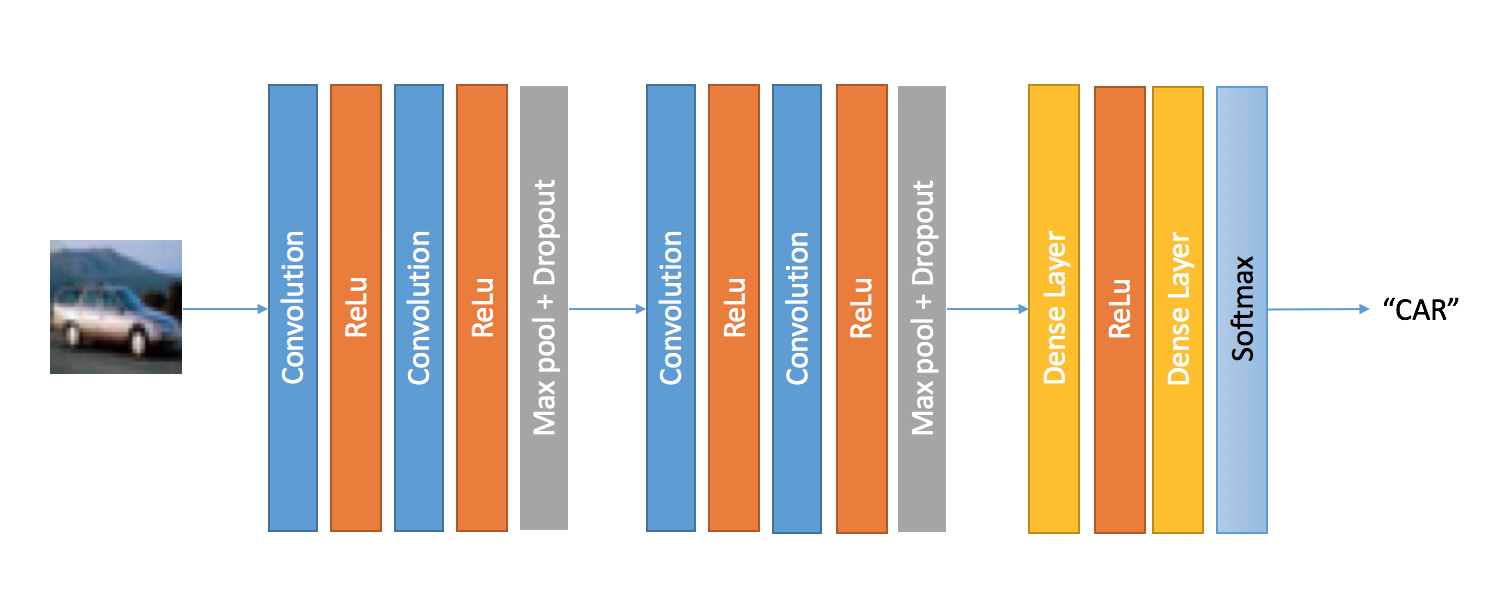
\includegraphics[width=0.9\textwidth]{images/cnn_arch.png} 
\caption{CNN Architecture}
\label{img:cnn_arch}
\end{figure}
\begin{table}[H]
\centering
\begin{tabular}{| l | l |} \hline
\textbf{Layer} & \textbf{Description}\\ \hline
Convolution & 3x3 32 filters, 3 stack \\ \hline
ReLu & ReLu Activation \\ \hline
Convolution & 3x3 32 filters 32 stack \\ \hline
ReLu & ReLu Activation \\ \hline
Max Pooling & 2x2 Max Pooling \\ \hline
Dropout & p=0.25 \\ \hline
Convolution & 3x3 64 filters, 32 stack \\ \hline
ReLu & ReLu Activation \\ \hline
Convolution & 3x3 64 filters 64 stack \\ \hline
ReLu & ReLu Activation \\ \hline
Max Pooling & 2x2 Max Pooling \\ \hline
Dropout & p=0.25 \\ \hline
Dense Layer & Linear Activation \\ \hline
ReLu & ReLu Activation \\ \hline
Dropout & p=0.5 \\ \hline
Dense Layer & Linear Activation \\ \hline
SoftMax Layer & 10 class output \\ \hline
\end{tabular}
\caption{CNN Layer Description}
\label{tab:cnn_layers}
\end{table}

\subsubsection*{Convolution Layer}
This is a key layer in CNN which performs the convolution on the previous layer outputs with convolutional filters. Convolution filter parameters are learnt during the training process using back propagation. This, unlike hand picked parameters in SIFT/HOG feature extraction techniques, is learnt using training data and determines the best possible features. Each level of convolutional layers extract different types of features. For example, first convolution layer extracts low level features like edges, lines, color gradients. 
\subsubsection*{ReLu Layer}
ReLu stands for Rectified Linear Units ($f(x)=max(0,x)$). Earlier neural networks used Sigmoid ($f(x) = (1+e^{-x})^{-1}$) or hyperbolic tangent functions. These functions have saturating  properties. ReLu has non-saturating properties and found to converge faster.
\subsubsection*{Max Pool + Dropout}
Pooling layers  reduces the variance and perform sub-sampling operation in the neural network. These layers can pick the max, min, average or l2 norm of the given window of inputs.
Dropout layer is reduced the overfitting in fully connected layers. 
\subsubsection*{Softmax layer}
This is similar to sigmoid function but with multi-class output in mind. This can be defined as: (x and w are vectors)
\[
P(y=j|x)=\frac{e^{x^Tw_j}}{\sum_{k=1}^{K}e^{x^Tw_k}}
\]

%%%%%%%%%%%%%%%%%%%%%%%%%%%%%%%%%%%%%%%%%%%%%%%%%%%%%%%%%%%%%%%%
\section{Methodology}
Following sections explain the methodologies used in different classification algorithms.
\subsubsection*{AdaBoost - Random Forest and SVM}
Figure \ref{img:flowchart_learning} represents the approach in learning algorithm and model selection. 
\begin{itemize}
\item Training data (HOG or BOF features) are normalized based mean and standard deviation of each features
\item From normalized features for training data, 3 cross validation sets are created. Every time, X-train is randomly shuffled and 85\% is named as new training portion and remaining 15\% is named as validation data. 
\item These data are stored in numpy files on network mounted drives (to be easily accessed by clusters)
\item IPython parallel and starcluster are used to submit the jobs to AWS cloud cluster and run the learning algorithms on the cloud in parallel. 
\item Once all the runs are completed, results are compared. Parameter with higher accuracy on validation data is considered best model. Overfitting is also handled by checking the difference between train and validation set accuracy numbers. Higher the difference, higher the overfitting.
\item With the best parameters from previous step, complete original training data is used to train the model and test the performance on test data (which was used until this step!).
\end{itemize}
\subsubsection*{Convolutional Neural Networks} 
Convolutional Neural Networks are really compute intensive and we need to get the things right in the first run, otherwise the run time is wasted and if we run on AWS, we will be spending a lot of money as well. g2.xlarge AWS instance is the basic 1GPU 8VCPU instance in AWS and costs 70 cents/hour. One run for 200 epochs takes 26 hours and costs \~\$20.

Keras support CIFAR-10 datasets really well and has plugins to directly decode the dataset. Train and Test data are collected from keras numpy dataset and features are normalized to have zero mean and unit variance. These data are provided for training and Neural Network trains using back propagation and Stochastic Gradient Descent. This is carried out several times to fit the model better. Care should be taken to monitor the overfitting of the model.



%%%%%%%%%%%%%%%%%%%%%%%%%%%%%%%%%%%%%%%%%%%%%%%%%%%%%%%%%%%%%%%%
\section{Implementation}
\subsection{Feature Space}\label{sec:feature_space}
CIFAR-10 dataset has 60,000 images, each with 32x32 pixels and RGB channels. These images are split into 50,000 train and 10,000 test images. Each pixel is represented by an unsigned integer number (0-255). Therefore each image has 32x32x3 = 3072 features. 
\subsection{Preprocessing and Feature Extraction}
3072 features directly obtained from image are not very useful, as they are mere rgb values and don't really contain the information about the object represented in the image. Very basic things, like a blue sky in most part of the image, might be helpful to classify airplanes (assuming that all airplanes pictures are taken while they are flying). In general, pixel values are highly correlated and don't account for scaling, rotation and translation of objects in the image. They don't even contain useful information about the shape of the object. This brings the necessity for alternate feature extraction techniques and look for robust features techniques to address these issues. SIFT and HOG are few standard feature extraction techniques in the computer vision literature and have their own advantages.
\subsubsection*{SIFT and Bag of Features}
SIFT\cite{ref:sift} features are invariant to scaling, rotation and translation. In the first step, keypoints are extracted in the gray scale image and in the latter step 128 dimensional descriptors are determined using 16x16 neighborhood around keypoint. So each SIFT keypoints have 128 dimensional and represent some key features in the image. The first step, keypoint extraction, is an important step which bring the invariant property to these features. Laplacian through Difference of Gaussian of image pyramids are used to detect keypoints. It is easy to match two images given their keypoints. Using these features directly is not a good approach, rather use bag of features approach suggested by \citet{ref:bof} and bag these features into 50 bags to get a 50 dimensional feature vector for each image.
\subsubsection*{Histogram of Gradients}
Histogram of Gradients mentioned above in section \ref{sec:hog_lit} explains the theory behind HOG feature extraction technique. Using 9 orientations,  8x8 pixels per cell,  3x3 cells per block; we get 324 dimensional feature vector for each images.
\subsection{Training, Validation and Model Selection}
Using features mentioned in section \ref{sec:feature_space}, SVM and RF+AdaBoost models are trained. Test set is isolated from the training process. Out of 50,000 training samples, three set of training and cross validation samples are created. To do this, samples are randomly shuffled and separated into 85\% training and 15\% cross validation set. Three such sets are independently trained on all the parameters of training algorithms. Best performing parameters are picked based on performance on cross validation dataset and considered as suitable parameters for training process. These parameters are then used to train the algorithm on complete training dataset and evaluated on original testing dataset. Performance on testing dataset is evaluated and represented as confusion matrix and precision and recall scores for better clarity and judgment.





%%%%%%%%%%%%%%%%%%%%%%%%%%%%%%%%%%%%%%%%%%%%%%%%%%%%%%%%%%%%%%%%
\section{Final Results}\label{sec:final_results}
\subsection{Results with BOF features}
This section illustrates the performance of different training algorithms on BOF features.
\subsubsection{BOF with Random Forest}
Figure \ref{img:rf_cv_bow} shows the variation of validation accuracy for every grid search parameters. First row represents the validation accuracy of number of estimators, second represents learning rate, third represents max depth, and the last one represents maximum number of features. From the plots, maximum number of features don't affect the accuracy a lot, whereas learning rate impacts the most. lower the learning rate, higher the accuracy.
\begin{figure}[H]
\centering
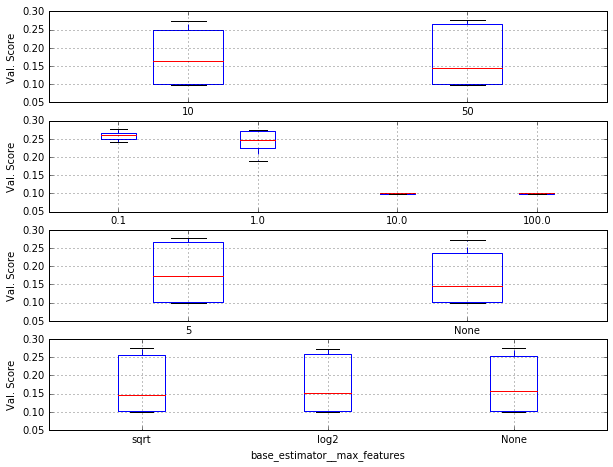
\includegraphics[width=0.9\textwidth]{images/rf_cv_bow.png} 
\caption{Grid Search Results for BOF with Random Forest}
\label{img:rf_cv_bow}
\end{figure}
Figure \ref{img:rf_cm_bow} represents the confusion matrix of BOF features classified using random forest and adaboost. The performance is very very poor and diagonal entries are lighter than few of the off-diagonal entries. This mean a severe mis-classification. 
\begin{figure}[H]
\centering
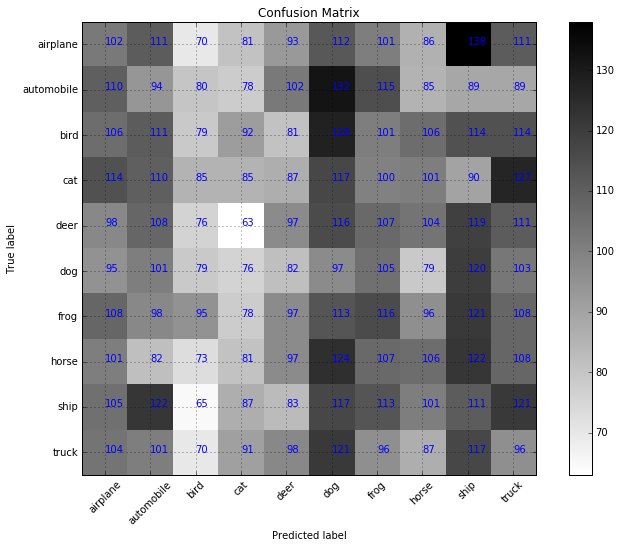
\includegraphics[width=0.9\textwidth]{images/rf_cm_bow.png} 
\caption{Confusion Matrix for BOF with Random Forest}
\label{img:rf_cm_bow}
\end{figure}
\paragraph{Grid Search Results}
Following are the grid search results using BOF features with Random Forest and AdaBoost classifier.  There is a clear sign of overfitting, train accuracy is much higher than validation accuracy. But, this was the best performing set out of all combinations and other iterations had poor accuracy as well as higher overfitting.
\begin{itemize}
\item validation set accuracy: 0.27173 (+/-0.00069) 
\item train set accuracy: 0.40913 (+/-0.00100)
\item n estimators: 50
\item learning rate: 1.0
\item rf max depth: 5
\item rf max features: sqrt
\end{itemize}


\subsubsection{BOF with SVM}
Figure \ref{img:svm_cv_bow} shows the variation of validation accuracy for every grid search parameters. First row represents the validation accuracy of kernels, second represents C and the last represents gamma. Interesting thing to note is that linear kernel overall performed better than rbf kernel. The best classifier noted below is one outlier in the batch.
\begin{figure}[H]
\centering
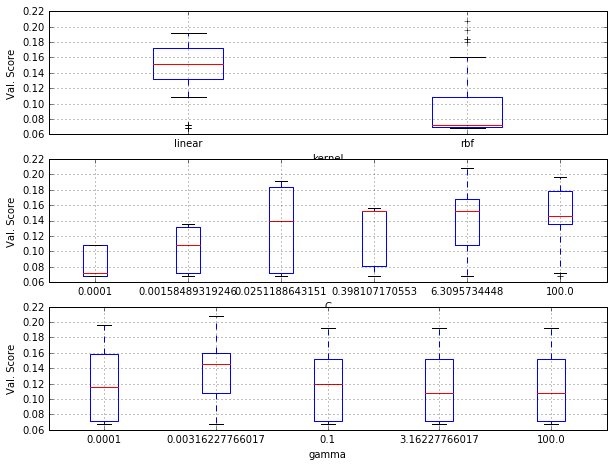
\includegraphics[width=0.9\textwidth]{images/svm_cv_bow.png} 
\caption{Grid Search Results for BOF with SVM}
\label{img:svm_cv_bow}
\end{figure}
\paragraph{Grid Search Results}
\begin{itemize}
\item validation set accuracy: 0.18800 (+/-0.00400) 
\item train set accuracy: 0.40311 (+/-0.00567)
\item kernel: rbf
\item C: 100.0
\item gamma: 0.0001
\end{itemize}


\subsection{Results with HOG features}
This section illustrates the performance of different training algorithms on HOG features.

\subsubsection{HOG with Random Forest}
Figure \ref{img:rf_cv_hog} shows the variation of validation accuracy for every grid search parameters. First row represents the validation accuracy of number of estimators, second represents learning rate, third represents max depth, and the last one represents maximum number of features. From the plots, number of estimators don't affect the accuracy a lot, whereas learning rate impacts the most. Lower the learning rate, higher the accuracy.

\begin{figure}[H]
\centering
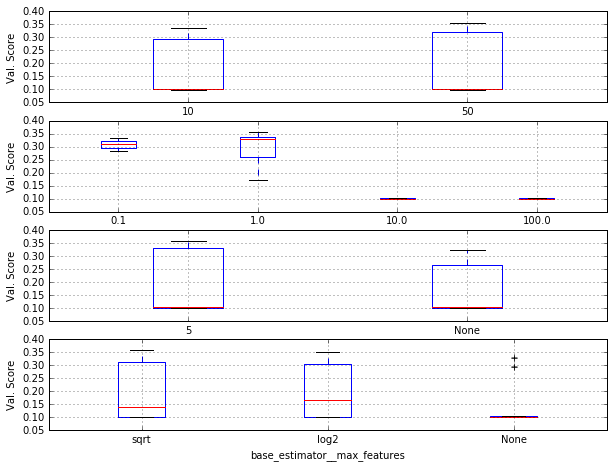
\includegraphics[width=0.9\textwidth]{images/rf_cv_hog.png} 
\caption{Grid Search Results for HOG with Random Forest}
\label{img:rf_cv_hog}
\end{figure}
Figure \ref{img:rf_cm_hog} shows the confusion matrix for this classifier. Diagonal entries are darker than off-diagonal entries, which is a sign of good classification compared to earlier methods. But the test accuracy numbers mentioned below show that the performance is just around 35\%. 
\begin{figure}[H]
\centering
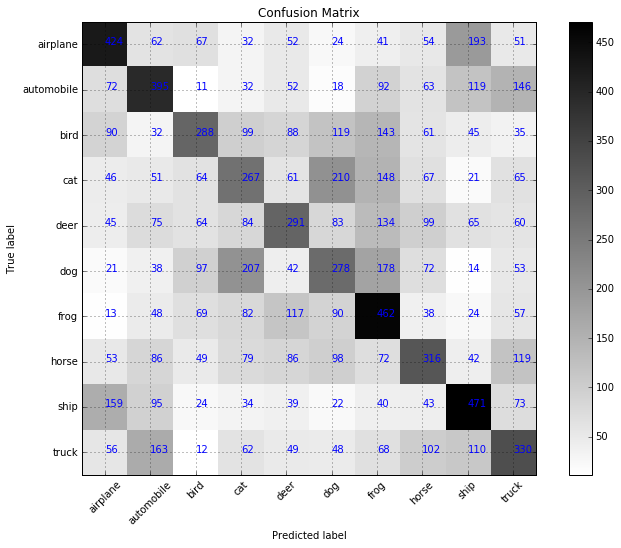
\includegraphics[width=0.9\textwidth]{images/rf_cm_hog.png} 
\caption{Confusion Matrix for HOG with Random Forest}
\label{img:rf_cm_hog}
\end{figure}
\paragraph{Grid Search Results}
\begin{itemize}
\item validation set accuracy: 0.34899 (+/-0.00395) 
\item train set accuracy: 0.49166 (+/-0.00054)
\item n estimators: 50 
\item learning rate: 1.0
\item rf max depth: 5
\item rf max features: sqrt
\end{itemize}
\paragraph{Classification Statistics}
Following table shows the classification results from the best classifier (obtained form grid search) \\
\begin{table}[H]
\centering
\begin{tabular}{| r | r | r | r | r |}
\hline
    & precision &   recall & f1-score &  support\\
 \hline
   airplane    &   0.43    &  0.42   &   0.43    &  1000\\
 automobile&       0.38     & 0.40    &  0.39  &    1000\\
       bird    &   0.39   &   0.29   &   0.33   &   1000\\
        cat   &    0.27    &  0.27   &   0.27   &   1000\\
       deer  &     0.33   &   0.29   &   0.31   &   1000\\
        dog  &     0.28   &   0.28    &  0.28    &  1000\\
       frog    &   0.34   &   0.46    &  0.39    &  1000\\
      horse   &    0.35 &     0.32   &   0.33  &    1000\\
       ship    &   0.43   &   0.47    &  0.45    &  1000\\
      truck     &  0.33   &   0.33    &  0.33    &  1000\\
\hline
avg / total     &  0.35 &     0.35 &     0.35 &    10000\\
\hline
\end{tabular}
\caption{Classification result of Random Forest + AdaBoost with HOG features}
\label{tab:rf_cs_hog}
\end{table}

\subsubsection{HOG with SVM}
Figure \ref{img:svm_cv_hog} shows the variation of validation accuracy for every grid search parameters. First row represents the validation accuracy of kernels, second represents C and the last represents gamma. Interesting thing to note is that linear kernel overall performed better than rbf kernel. The best classifier noted below is one outlier in the batch. One other interesting behavior to note is that gamma 0.0031 has a best performance and it drops on either sides of this value.
\begin{figure}[H]
\centering
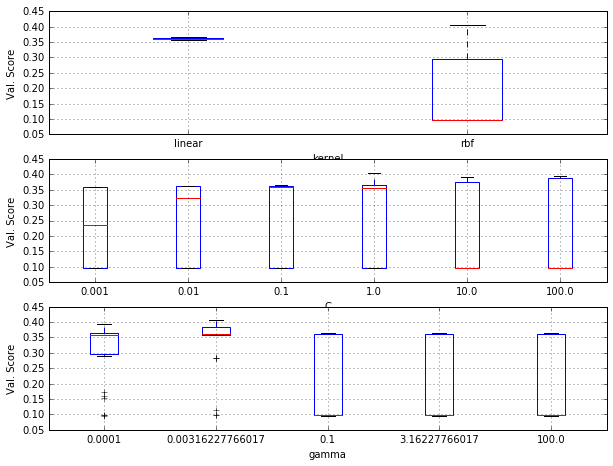
\includegraphics[width=0.9\textwidth]{images/svm_cv_hog.png} 
\caption{Grid Search Results for HOG with SVM}
\label{img:svm_cv_hog}
\end{figure}
Figure \ref{img:svm_cm_hog} shows the confusion matrix for this classifier. The darker diagonal entries compared to off-diagonal entries are a good sign of performance and following section on classification statistics shows the 42\% accuracy on test set.
\begin{figure}[H]
\centering
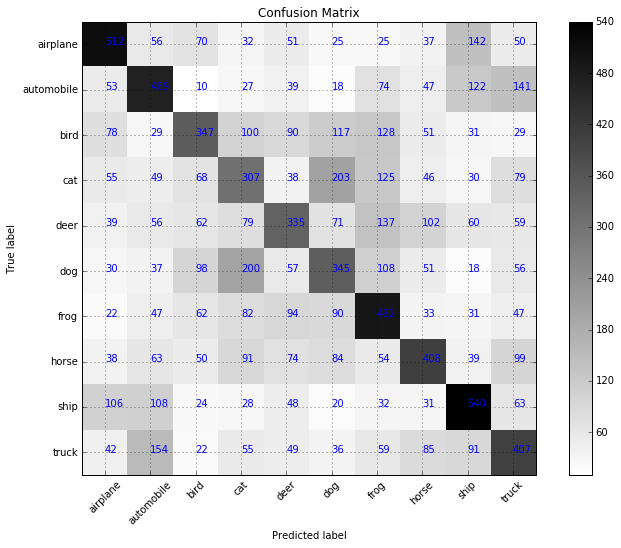
\includegraphics[width=0.9\textwidth]{images/svm_cm_hog.png} 
\caption{Confusion Matrix for HOG with SVM}
\label{img:svm_cm_hog}
\end{figure}
\paragraph{Grid Search Results}
\begin{itemize}
\item validation set accuracy: 0.40571 (+/-0.00014)
\item train set accuracy: 0.63372 (+/-0.00097)
\item kernel: rbf
\item C: 1.0
\item gamma: 0.00316
\end{itemize}
\paragraph{Classification Statistics}
Following table shows the classification results from the best classifier (obtained form grid search) \\
\begin{table}[H]
\centering
\begin{tabular}{| r | r | r | r | r |}
\hline
    & precision &   recall & f1-score &  support\\
 \hline
   airplane  &     0.53    &  0.51 &     0.52    &  1000\\
 automobile   &    0.44  &    0.47   &   0.45  &    1000\\
       bird     &  0.43  &    0.35 &     0.38   &   1000\\
        cat     &  0.31  &    0.31   &   0.31  &    1000\\
       deer   &    0.38   &   0.34 &     0.36   &   1000\\
        dog    &   0.34   &   0.34   &   0.34  &    1000\\
       frog   &    0.40   &   0.49    &  0.44   &   1000\\
      horse &      0.46  &    0.41  &    0.43  &    1000\\
       ship    &   0.49   &   0.54    &  0.51   &   1000\\
      truck    &   0.40  &    0.41    &  0.40  &    1000\\
\hline
avg / total    &   0.42    &  0.42    &  0.41   &  10000\\
\hline
\end{tabular}
\caption{Classification result of SVM with HOG features}
\label{tab:svm_cs_hog}
\end{table}

\subsection{Results with CNN}
Figure \ref{img:cnn_cm} shows the confusion matrix for CNN classifier. As we can note that diagonal entries are much darker compared to any classifiers before, this represents a good classification. Classification report mentioned below reflects the same.
\begin{figure}[H]
\centering
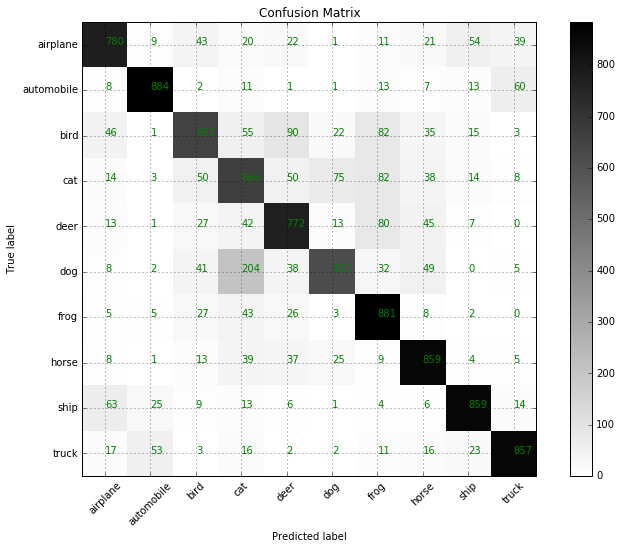
\includegraphics[width=0.9\textwidth]{images/cnn_cm.png} 
\caption{Confusion Matrix for CNN 50 epochs}
\label{img:cnn_cm}
\end{figure}
\paragraph{Classification Statistics}
Following table shows the classification results from CNN in 50 epochs: \\
\begin{table}[H]
\centering
\begin{tabular}{| r | r | r | r | r |}
\hline
    & precision &   recall & f1-score &  support\\
\hline
   airplane   &    0.81 &     0.78   &   0.80&      1000\\
 automobile&       0.90  &    0.88 &     0.89   &   1000\\
       bird     &  0.75   &   0.65  &    0.70    &  1000\\
        cat     &  0.60   &   0.67    &  0.63   &   1000\\
       deer    &   0.74   &   0.77   &   0.76   &   1000\\
        dog     &  0.81   &   0.62    &  0.70   &   1000\\
       frog    &   0.73   &   0.88   &   0.80    &  1000\\
      horse  &     0.79   &   0.86  &    0.82  &    1000\\
       ship    &   0.87    &  0.86   &   0.86   &   1000\\
      truck    &   0.86    &  0.86   &   0.86   &   1000\\
\hline
avg / total   &    0.79   &   0.78  &    0.78   &  10000\\
\hline
\end{tabular}
\caption{Classification results of CNN}
\label{tab:cnn_cs}
\end{table}

\paragraph{Kaggle Competition Result}
CIFAR-10 Kaggle competition has ended last year and no new entries are accepted in the leader board. But the best performance result from this project can be placed 52 out of 231 entries in the leader board.




%%%%%%%%%%%%%%%%%%%%%%%%%%%%%%%%%%%%%%%%%%%%%%%%%%%%%%%%%%%%%%%%
\section{Interpretation}
Section \ref{sec:final_results} shows the results of all the experiments. Since the dataset is huge, it takes quiet some time to run on local machines. Typical grid searches on random forest were taking 13-15 hours on MacBook pro laptop with i7 processor, 8GB RAM and SSD storage. SVM runs were taking very long time and crashed in between due to machine issues. Later, all the runs were run on 40-70 clusters on Amazon Web Services (AWS). 

As Figure \ref{img:rf_cm_bow} shows, BOF features are very bad. This is mainly because of features used to create the bags. SURF and ORB features couldn't be extracted. SIFT features were extracted with lot of modifications to sigma and threshold parameters. I believe this is the reason for bad features and and hence worst performance on BOF features with AdaBoost+Random Forest as well as SVM classifiers.

HOG Dense features tend to perform much better than BOF features. As in table \ref{tab:rf_cs_hog} and table \ref{tab:svm_cs_hog}, classifiers reach upto 42\% accuracy on test dataset. AdaBoost+RF classifier gives ~35\% accuracy on test set and slightly below the SVM results. But training time for AdaBoost+RF classifier grid search was three times lesser than SVM grid search.

CNN results outperform all other results by factor of two. With 50 epochs, I gave got close to 78\% accuracy on test set and clearly see a scope to improve this results with more processing power and GPUs. Just for a sake of curiosity, I saved the weights for all epochs and tested their performance on test sets. Test set error was 75\% for 25 epochs, later improved to 76\% at 35 epochs and finally to 78.3\% for 50 epochs. Each epochs took 5800s for training and 940s for testing on CPUs, but took only 519s for training and 41s for testing on Nvidia K520 GPUs.





%%%%%%%%%%%%%%%%%%%%%%%%%%%%%%%%%%%%%%%%%%%%%%%%%%%%%%%%%%%%%%%%
\section{Summary and Conclusions}
Performance and results clearly indicate that CNN is the best classifier for this case. It is possible to improve the performance even further by using real time data augmentations and deeper convolutional networks. Some of the top performers in Kaggle leader board have shared their network architectures and support my idea. Top performers on Kaggle use deeper VGG nets with ZCA whitened and normalized images to address features correlation in images and have achieved close to ~95\% accuracy. 

Training deep neural networks might be time and compute intensive. So, some literature suggests to use trained models as feature extractors. The features might not be optimal, but assured to give better performance than existing feature extraction techniques. These features can be tapped from dense output or intermediate convolutional layers. Logistic regression or SVM on these features can give good results. I look forward to try these techniques in the winter break and compare them with my results.

On the other hand, this project is a great experience to handle big data and implementing machine learning algorithms efficiently. Many existing algorithms work well on a smaller dataset, but don't scale well with larger data. Thinking of how can it be implemented in parallel is crucial and great learning experience. Handling cloud based computing resources and open source tools are equally great experiences. Over the course of the project, I have fixed couple of bugs in open source tools and contributed to their betterment.


%%%%%%%%%%%%%%%%%%%%%%%%%%%%%%%%%%%%%%%%%%%%%%%%%%%%%%%%%%%%%%%%
\bibliography{references}
%\bibliographystyle{unsrt}


%%%%%%%%%%%%%%%%%%%%%%%%%%%%%%%%%%%%%%%%%%%%%%%%%%%%%%%%%%%%%%%%
\newpage
\begin{center}
\begin{LARGE}
\textbf{Appendix}
\end{LARGE}
\end{center}
\appendix
\section{Software Tools}
Following softwares and toolsare used in this project:
\begin{itemize}
\item \textbf{Scikit-Learn}: Python based machine learning library. Has implementations of SVM, Adaboost, Random Forest etc,.
\item \textbf{Scikit-Image}: Another python based library from Scikit-learn developers, useful to extract image features.
\item \textbf{Keras}: Theano based deep learning library with python support. Has all basic layers, like convolutional layer, ReLu, Dropout etc,.
\item \textbf{IPython and IPython Parallel}: Browser based interactive python shell. Supports cluster computing for parallel running jobs through ipcluster.
\item \textbf{OpenCV}: Open Computer Vision library with Python support. Used to extract SIFT, SURF and ORB features.
\item \textbf{Starcluster}: MIT open source tool to manage AWS clusters.
\item \textbf{AWS}: Amaon Web Services. Cloud computing platform and useful to run compute intensive learning algorithms.
\item \textbf{Bitbucket}: Code version management and repository.
\end{itemize}

\end{document}
This is never printed